\chapter{Monte Carlo and Data}
\label{ch:mc_data}

The search for semi-visible jets via s-channel production presented in the following chapters is performed with an integrated luminosity of 139 \fb~of proton-proton collision data collected by the ATLAS detector during Run 2 (2015 - 2018). The full Run 2 dataset is used for the final interpretation. Monte Carlo (MC) simulations of background processes and the semi-visible jet signal process are used in the development of the analysis strategy, and in the final interpretation to set limits on the observed cross-section of the signal model. This chapter will provide details about the full Run 2 dataset, and the background MC simulations, and the signal MC simulations used in this search. 

\section{Data}
The 139 \fb~integrated luminosity of proton-proton collision data used for physics analyses are required to pass a set of data quality checks. In Run 2 94\% of the $pp$ collisions delivered by the LHC were successfully recorded by the ATLAS experiment, as illustrated in Figure~\ref{fig:atlas_grl}. 95\% of the data recorded by the ATLAS experiment was marked as ``good for physics", resulting in 139 \fb~of integrated luminosity. Events are rejected if they are corrupted or incomplete, or if they were recorded during a subsystem malfunction. 

\begin{figure}
        \centering
	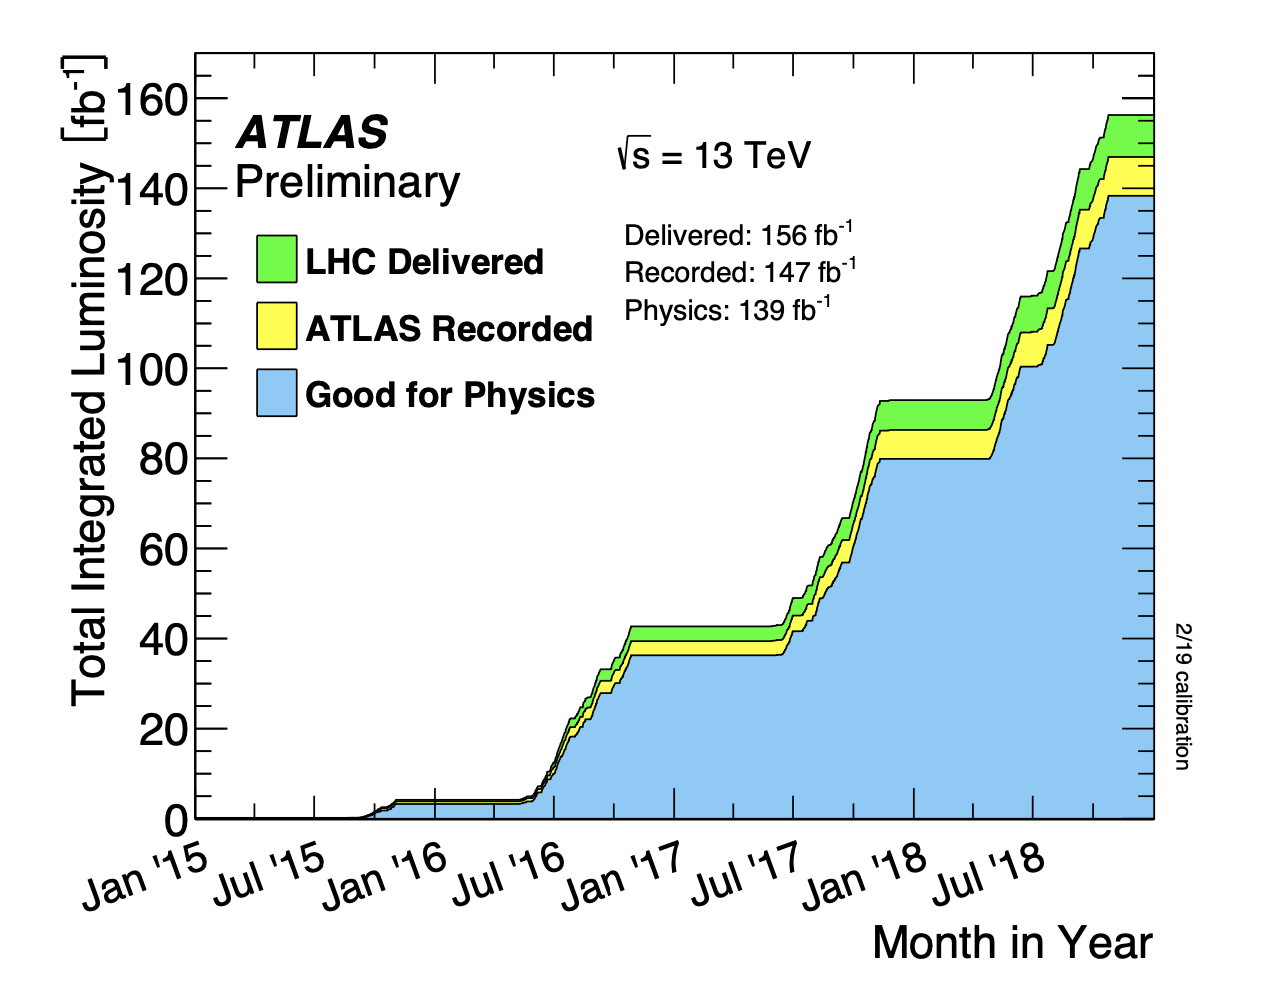
\includegraphics[width=0.62\textwidth]{figures/ch6/atlas_grl}
	\caption{Integrated luminosity for the ATLAS experiment as a function of time during Run 2 \cite{atlas_grl}
	\label{fig:atlas_grl}}
\end{figure}

Events for this analysis are further required to pass a single-jet trigger selection, where events are required to have a jet at trigger-level with a \pt~that exceeds a certain value. 
The lowest \pt~unprescaled\footnote{An unprescaled trigger records every event that meets the trigger requirement. A prescaled trigger only records a fraction of events that meet the trigger requirement.} single jet trigger threshold for each period is as follows: 

\begin{itemize}
\item 2015: \pt $\geq$ 360 GeV
\item 2016 \& 2017:  \pt $\geq$ 380 GeV
\item 2018:  \pt $\geq$ 420 GeV
\end{itemize}

A post-trigger selection of jet \pt~> 450 GeV ensures all these triggers are fully within their efficiency plateaus. The jet collection used is anti-$k_t$ EM particle flow jets with a radius parameter of R = 0.4, also referred to as small-R jets. \par

Due to the variance in visible and invisible momenta due to the \rinv~parameter of the signal model, many signals also have significant \met.
The use of a \met~trigger to select events was considered, and the single jet approach described here was found to preserve more signal events across the grid, particularly in the high resonance mass and low ~\rinv~region of phase space. These studies are documented in Appendix~\ref{app:trigger}.\par

The data are subject to a blinding strategy throughout the analysis design so as to mitigate analyzer-induced bias. 
Blinded and unblinded region definitions are described further in Section~\ref{sec:eventsel}.

\section{Simulation}
\label{sec:simulation}

Simulated events are generated with a variety of Monte Carlo (MC) generator processes that run in stages. The $pp$ hard scatter physics process is simulated, and the final state particles are subsequently showered and decayed. This full description of the event is then propagated through a detailed detector simulation based on GEANT4~\cite{Agostinelli:2002hh}. The MC simulation is weighted to match the distribution of the average number of interactions per bunch crossing $\mu$ observed in collision data.\par

All simulated samples included in this analysis were produced with three different MC campaigns: $\texttt{mc20a}$ corresponds to 2015-2016 data-taking conditions, $\texttt{mc20d}$ to 2017, and $\texttt{mc20e}$ to 2018. These three campaigns are weighted to the integrated luminosities of their respective data-taking periods and combined to produce simulation for the entire Run 2 dataset. Simulated events are reconstructed with the same algorithms run on collision data. 


\subsection{Simulated Backgrounds}
\label{subsec:bkg_mc}

Although the final background estimation is data-driven, background MC is studied for analysis optimization and machine learning tool development.\par

Dijet QCD is the dominant background process. QCD is simulated with \textsc{Pythia8}~\cite{pythia}, and generated in approximate slices of \pt, to ensure high statistics across the momentum spectrum. The slices are then reweighted using MC generated event weights to create a physical distribution. Figure~\ref{fig:jzslices} illustrates the 8 momentum slices used in this analysis.

\begin{figure}
        \centering
	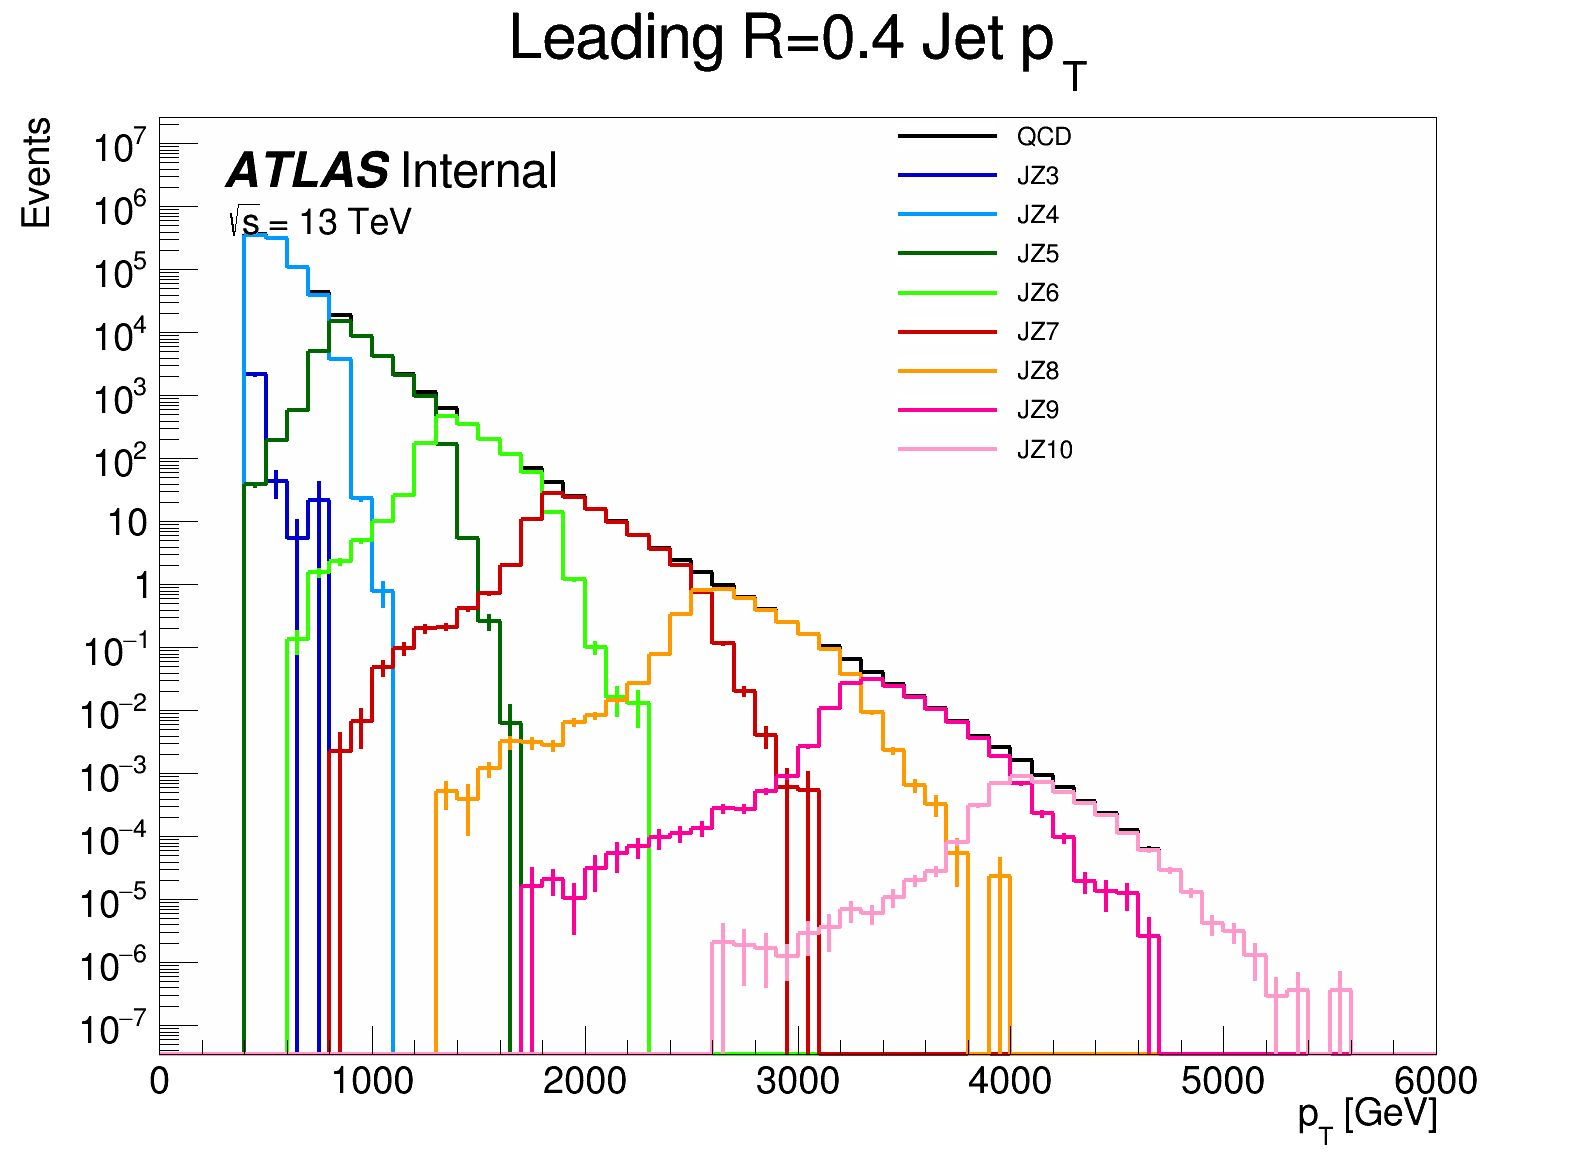
\includegraphics[width=0.49\textwidth]{figures/ch6/jz_slices}
	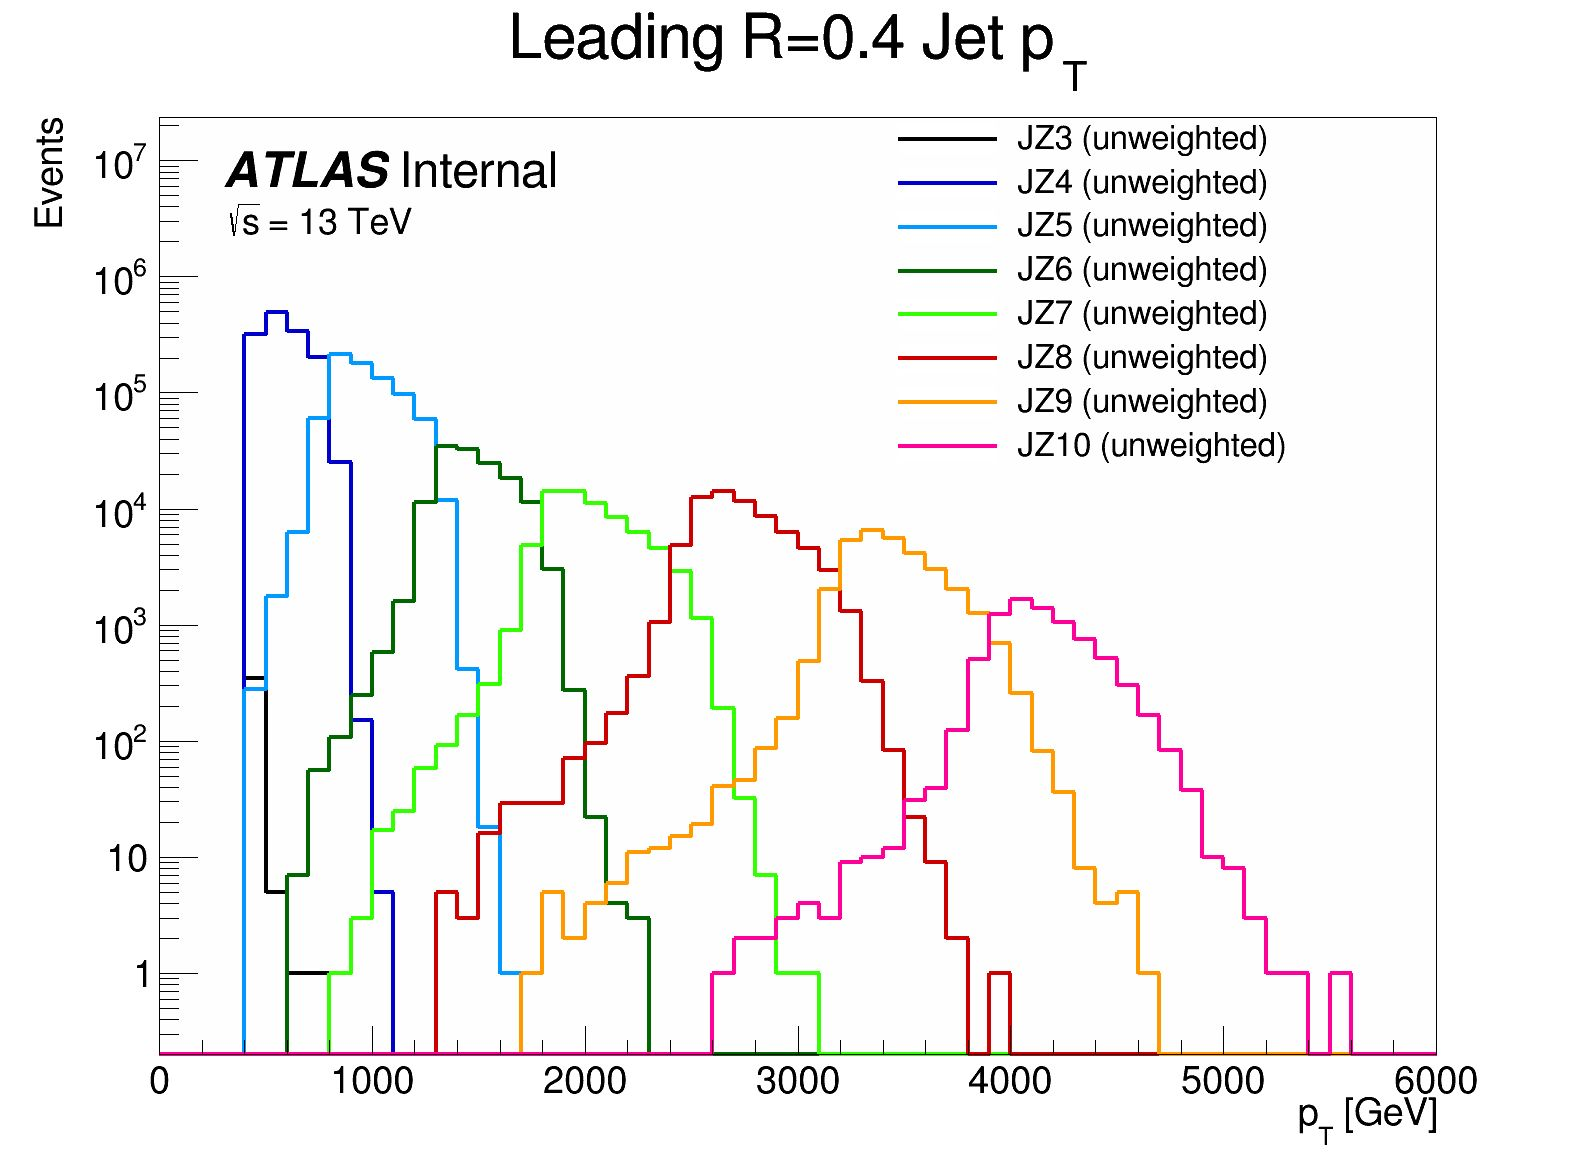
\includegraphics[width=0.49\textwidth]{figures/ch6/jz_slices_uw}
	\caption{The transverse momentum slices of the QCD MC simulation, overlayed to show how they come together to create a smooth distribution (left) once weighted properly. The original unweighted distribution is shown on the right, illustrating the enhanced statistics for the high \pt~range. 
	\label{fig:jzslices}}
\end{figure}

Due to presence of \met in the SVJ signals, additional MC background processes are required to create a full picture of the relevant background. 
The $Z\rightarrow \nu\nu$ process contributes to the background due to its high missing energy. 
Leptonic W/Z decays and W/Z+jets are also included as they can contribute both additional missing energy and significant hadronic activity.
Single top and $t\bar{t}$ processes are also considered for their contribution to hadronic activity.
After the analysis \textit{preselection}\footnote{A preselection is a set of cuts on physical observables used to isolate a collection of events which are most likely to contain the desired signal. The preselection for this analysis will be discussed in Section~\ref{sec:eventsel}} is applied to isolate events most relevant to the SVJ topology, the background composition is 76\% QCD, 12\% $W$+jets, 8\% top and $t\bar{t}$ processes, and 4\% $Z\rightarrow \nu\nu$.  
Figure~\ref{fig:bkg_mc} illustrates the background composition for the analysis.
The lower panel in Figure~\ref{fig:bkg_mc} illustrates the ratio between data (black) and the combined MC processes (grey).
While the agreement between data and MC is not perfect (ratio = 1.0 for all \met~ values), the difference is $<20$\% throughout the distribution.
This is within tolerance for this analysis, since the final background estimation will be data driven, and background MC is only needed for approximate modeling.
Analysis selections for high energy jets (discussed in Section~\ref{sec:eventsel}) create some sculpting in the $Z\rightarrow \nu\nu$ and $W$+jets distributions; however, the total \met~ distribution is smoothly falling so this is not an issue.

\begin{figure}
        \centering
	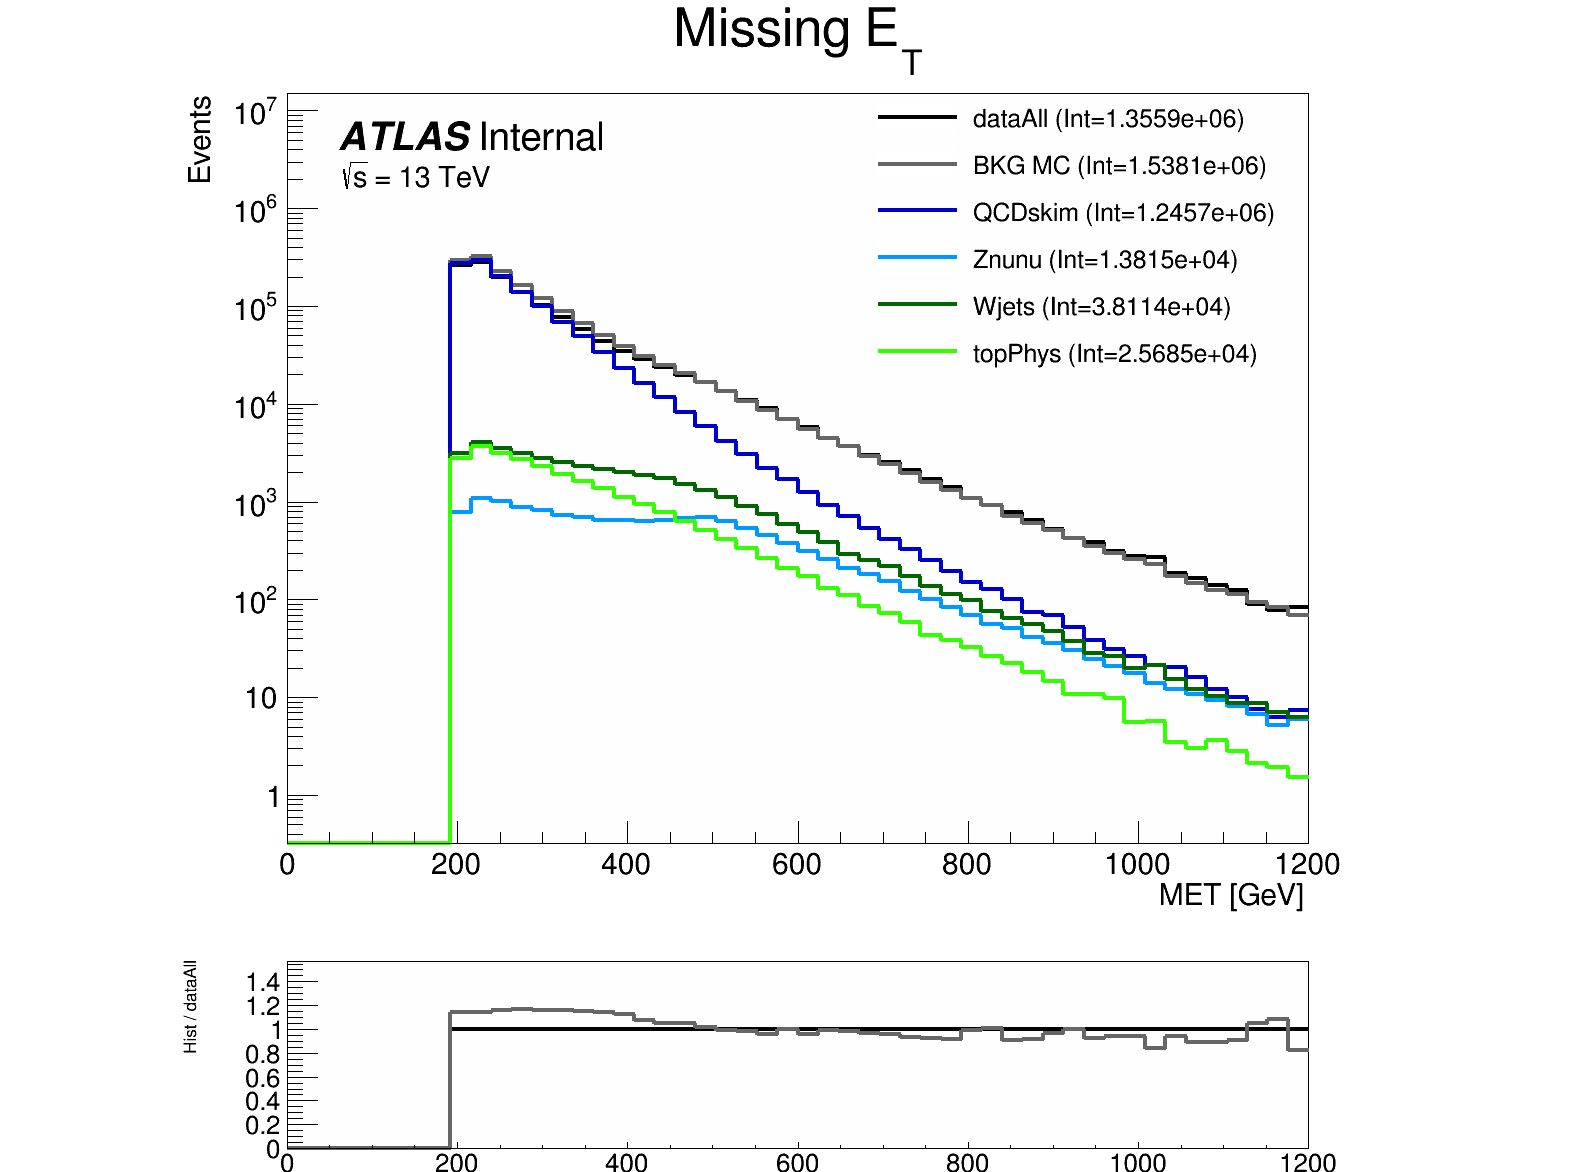
\includegraphics[width=0.55\textwidth]{figures/ch6/bkg_mc}
	\caption{Background processes relevant to the SVJ signal. 
	\label{fig:bkg_mc}}
\end{figure}

\subsection{Signal Simulation}
\label{subsec:signals}

The Hidden Valley (HV) signal model implementation is based on Ref~\cite{darkqcd}. 
The s-channel semi-visible jet model, which was described in Chapter~\ref{ch:theory}, is governed by a number of parameters. 
The mass of the mediator $m_{Z'}$ can be set, together with the couplings of the $Z'$ to the visible and dark quarks $g_q$ and $g_{q_D}$. 
The dark sector shower is governed by the number of dark colors $N_{c_D}$, the number of dark flavors $N_{f_D}$, and the dark sector confinement scale $\Lambda_D$. 
There is also the characteristic scale of the dark hadrons $m_{dark}$, determined by the mass of the dark quarks $m_{q_D}$. 
The characteristic scale determines the mass of the dark hadrons, which can be pseudoscalars $m_{\pi_D}$ or vectors $m_{\rho_D}$.
Finally, the average fraction of invisible particles in the final state jet is dictated by \rinv. 

%Our choices of these parameters are informed by the 2021 Snowmass report~\cite{snowmass}. 
The chosen parameters for this model were carefully selected in collaboration with theorists to be compatible with the new benchmarks established in the 2021 Snowmass process~\cite{snowmass}. 
The signal generation allows for up to two initial state radiation jets, and uses a jet-matching scheme described in Ref.~\cite{mlm} and implemented in Ref.~\cite{pythia} to match jets to the original partons.
%A notable remaining difference between the ATLAS s-channel and t-channel searches 

The choices of fixed parameters for the Pythia8 HV model are summarized in Table \ref{tab:model_fixed_params}.
A detailed discussion of these parameters and their implications on the dark shower topology can be found in Ref.~\cite{snowmass}. 
The mass choices for the dark quark and the dark hadrons are also summarized in Table \ref{tab:model_mdark}. 

\begin{table}
\centering
  \begin{tabular}{ |c|c| }
    \hline
    Parameter & Value \\
    \hline
     $N_{c_D}$ & 3.0 \\
     $g_{q_D}$& 1.0\\
     $\Lambda_D$ & 10.0\\
     $N_{f_D}$ & 2.0\\
    \hline
  \end{tabular}
  \caption{Fixed parameters in the Pythia8 HV model}
  \label{tab:model_fixed_params}
\end{table}

Note that the number of dark flavors differs from the Snowmass recommendation of $N_{f_D}$ = 4. 
This change is minimal in impact because \rinv~is set explicitly (rather than allowing it to arise naturally from the HV theory), and allows this ATLAS analysis result to remain comparable with the CMS semi-visible jets s-channel analysis \cite{cms_svj} and the ATLAS semi-visible jets t-channel analysis \cite{tchannel}. \par

\begin{table}
\centering
  \begin{tabular}{ |c|c| }
    \hline
    Parameter & Value [GeV] \\
    \hline
     $m_{\pi_D}$ & 17.0 \\
     $m_{\rho_D}$ & 31.77 \\ 
     $m_{q_D}$ & 10.0 \\ 
    \hline
  \end{tabular}
  \caption{Values for $m_{dark}$}
  \label{tab:model_mdark}
\end{table}

The mediator mass $m_{Z'}$ and the fraction of invisible particles in the final state \rinv~vary, and are used to define the search grid. $m_{Z'}$ varies between 2.0 TeV and 5.0 TeV, while~\rinv~ varies from 0.2 to 0.8. \rinv~values of 0.2, 0.4, 0.6, and 0.8 are generated for each $m_{Z'}$ mass point. Table \ref{tab:sig_grid} illustrates the signal grid and the associated cross-section for each signal.

\begin{table}
\centering
  \begin{tabular}{ |c|c| }
    \hline
    $m_{Z'}$ (GeV) & Cross section (fb)  \\
    \hline
     2000 &  252 \\
     2500 &  74.2 \\
     3000 &  24.5\\ 
     3500 &  8.83\\
     4000 &  3.49 \\ 
     5000 &  0.757 \\
    \hline
  \end{tabular}
  \caption{Mass points and cross sections of the SVJ search signal grid}
  \label{tab:sig_grid}
\end{table}

Samples are generated using 
\textsc{MadGraph5}~\cite{Alwall:2014hca} version 2.9.9 interfaced to 
\textsc{Pythia8.244p3}~\cite{pythia} for shower and hadronization with 
NNPDF23LO PDF~\cite{Butterworth:2015oua} and the 
ATLAS A14~\cite{Skands:2014pea} to tune the underlying event data.
